\documentclass[a4paper,12pt,twoside]{memoir}

% Castellano
\usepackage[spanish,es-tabla]{babel}
\selectlanguage{spanish}
\usepackage[utf8]{inputenc}
\usepackage[T1]{fontenc}
\usepackage{lmodern} % Scalable font
\usepackage{microtype}
\usepackage{placeins}

\RequirePackage{booktabs}
\RequirePackage[table]{xcolor}
\RequirePackage{xtab}
\RequirePackage{multirow}

% Links
\PassOptionsToPackage{hyphens}{url}\usepackage[colorlinks]{hyperref}
\hypersetup{
	allcolors = {red}
}

% Ecuaciones
\usepackage{amsmath}

% Rutas de fichero / paquete
\newcommand{\ruta}[1]{{\sffamily #1}}

% Párrafos
\nonzeroparskip

% Huérfanas y viudas
\widowpenalty100000
\clubpenalty100000

\let\tmp\oddsidemargin
\let\oddsidemargin\evensidemargin
\let\evensidemargin\tmp
\reversemarginpar

% Imágenes

% Comando para insertar una imagen en un lugar concreto.
% Los parámetros son:
% 1 --> Ruta absoluta/relativa de la figura
% 2 --> Texto a pie de figura
% 3 --> Tamaño en tanto por uno relativo al ancho de página
\usepackage{graphicx}

\newcommand{\imagen}[3]{
	\begin{figure}[!h]
		\centering
		\includegraphics[width=#3\textwidth]{#1}
		\caption{#2}\label{fig:#1}
	\end{figure}
	\FloatBarrier
}







\graphicspath{ {./img/} }

% Capítulos
\chapterstyle{bianchi}
\newcommand{\capitulo}[2]{
	\setcounter{chapter}{#1}
	\setcounter{section}{0}
	\setcounter{figure}{0}
	\setcounter{table}{0}
	\chapter*{#2}
	\addcontentsline{toc}{chapter}{#2}
	\markboth{#2}{#2}
}

% Apéndices
\renewcommand{\appendixname}{Apéndice}
\renewcommand*\cftappendixname{\appendixname}

\newcommand{\apendice}[1]{
	%\renewcommand{\thechapter}{A}
	\chapter{#1}
}

\renewcommand*\cftappendixname{\appendixname\ }

% Formato de portada

\makeatletter
\usepackage{xcolor}
\newcommand{\tutor}[1]{\def\@tutor{#1}}
\newcommand{\tutorb}[1]{\def\@tutorb{#1}}

\newcommand{\course}[1]{\def\@course{#1}}
\definecolor{cpardoBox}{HTML}{E6E6FF}
\def\maketitle{
  \null
  \thispagestyle{empty}
  % Cabecera ----------------
\begin{center}
  \noindent
\includegraphics[width=\textwidth]{cabeceraSalud}\vspace{1.5cm}%
\end{center}
  
  % Título proyecto y escudo salud ----------------
  \begin{center}
    \begin{minipage}[c][1.5cm][c]{.20\textwidth}
        
\includegraphics[width=\textwidth]{escudoSalud.pdf}
    \end{minipage}
  \end{center}
  
  \begin{center}
    \colorbox{cpardoBox}{%
        \begin{minipage}{.8\textwidth}
          \vspace{.5cm}\Large
          \begin{center}
          \textbf{TFG del Grado en Ingeniería de la Salud}\vspace{.6cm}\\
          \textbf{\LARGE\@title{}}
          \end{center}
          \vspace{.2cm}
        \end{minipage}
    }%
  \end{center}
  
    % Datos de alumno, curso y tutores ------------------
  \begin{center}%
  {%
    \noindent\LARGE
    Presentado por \@author{}\\ 
    en Universidad de Burgos\\
    \vspace{0.5cm}
    \noindent\Large
    \@date{}\\
    \vspace{0.5cm}
    %Tutor: \@tutor{}\\ % comenta el que no corresponda
    Tutor: \@tutor{} \\
  }%
  \end{center}%
  \null
  \cleardoublepage
  }
\makeatother

\newcommand{\nombre}{Inés Martos Barbero}
\newcommand{\nombreTutor}{Guirguis Zaki Guirguis Abdelmessih} 
\newcommand{\dni}{09106453V} 

% Datos de portada
\title{Aplicación web para el seguimiento de la actividad de las personas con enfermedad de Parkinson}
\author{\nombre}
\tutor{\nombreTutor}
\date{\today}


\begin{document}

\maketitle


\newpage\null\thispagestyle{empty}\newpage

%%%%%%%%%%%%%%%%%%%%%%%%%%%%%%%%%%%%%%%%%%%%%%%%%%%%%%%%%%%%%%%%%%%%%%%%%%%%%%%%%%%%%%%%
\thispagestyle{empty}


\noindent
\includegraphics[width=\textwidth]{cabeceraSalud}\vspace{1cm}

\noindent D. \nombreTutor, profesor del departamento de departamento, área de área.

\noindent Expone:

\noindent Que el alumno D. \nombre, con DNI \dni, ha realizado el Trabajo final de Grado en Ingeniería de la Salud titulado título del trabajo. 

\noindent Y que dicho trabajo ha sido realizado por el alumno bajo la dirección del que suscribe, en virtud de lo cual se autoriza su presentación y defensa.

\begin{center} %\large
En Burgos, {\large \today}
\end{center}

\vfill\vfill\vfill

% Author and supervisor
%\begin{minipage}{0.45\textwidth}
%\begin{flushleft} %\large
%Vº. Bº. del Tutor:\\[2cm]
%D. \nombreTutor
%\end{flushleft}
%\end{minipage}
%\hfill
%\begin{minipage}{0.45\textwidth}
%\begin{flushleft} %\large
%Vº. Bº. del Tutor:\\[2cm]
%D. \nombreTutorb
%\end{flushleft}
%\end{minipage}
%\hfill

\vfill

% para casos con solo un tutor comentar lo anterior
% y descomentar lo siguiente
Vº. Bº. del Tutor:\\[2cm]
D. \nombreTutor


\newpage\null\thispagestyle{empty}\newpage




\frontmatter

% Abstract en castellano
\renewcommand*\abstractname{Resumen}
\begin{abstract}

Los problemas motores característicos de la Enfermedad de Párkinson (EP) afectan significativamente la función de la marcha, provocando episodios de congelación de la marcha en las etapas más críticas. Esto repercute considerablemente en la calidad de vida de las personas con EP.

Los dispositivos de monitorización disponibles para esta enfermedad son caros y escasos, y son aún menos los enfocados en analizar los parámetros de la marcha. La recopilación y análisis de esta información son esenciales para facilitar la toma de decisiones objetivas e informadas por parte de los profesionales sobre la modificación del tratamiento y adaptación de terapias.

Continuando con un proyecto anterior, cuyo objetivo era proporcionar una herramienta de apoyo en el ámbito clínico y de ayuda para pacientes, se han realizado pequeñas mejoras en el hardware del dispositivo utilizado para el registro de datos y se ha desarrollado un software, concretamente un sitio web. Este avance ha permitido el funcionamiento inalámbrico del dispositivo mediante el empleo de Bluetooth para la comunicación con el servidor web. La transmisión de datos se realiza en tiempo real, lo que permite su visualización desde una interfaz simple que también posibilita la gestión de la recogida de datos. La innovación de la plataforma web consiste en permitir tanto a profesionales como a pacientes acceder de forma sencilla a la información más relevante.

\end{abstract}

\renewcommand*\abstractname{Descriptores}
\begin{abstract}
Enfermedad de Párkinson, problemas motores, congelación de la marcha, análisis de la marcha, monitorización, aplicación web, software, datos en tiempo real, comunicación inalámbrica, Bluetooth, innovación tecnológica.
\end{abstract}

\clearpage

% Abstract en inglés
\renewcommand*\abstractname{Abstract}
\begin{abstract}
The characteristic motor problems of Parkinson's Disease (PD) significantly affect gait function, causing freezing of gait episodes in the most critical stages. This considerably impacts the quality of life of people with PD.

The monitoring devices available for this disease are expensive and scarce, and even fewer focus on analyzing gait parameters. The collection and analysis of this information are essential to facilitate objective and informed decision-making by professionals regarding treatment modification and therapy adaptation.

Continuing with a previous project, whose goal was to provide a support tool in the clinical setting and aid for patients, small improvements have been made to the hardware of the device used for data recording, and software has been developed, specifically a website. This advancement has enabled the wireless operation of the device through the use of Bluetooth for communication with the web server. Data transmission occurs in real-time, allowing its visualization from a simple interface that also enables the management of data collection. The innovation of the web platform lies in allowing both professionals and patients to easily access the most relevant information.


\end{abstract}

\renewcommand*\abstractname{Keywords}
\begin{abstract}
Parkinson's Disease, motor problems, freezing of gait, gait analysis, monitoring, website, software, real-time data, wireless communication, Bluetooth, technological innovation.
\end{abstract}

\clearpage

% Indices
\tableofcontents

\clearpage

\listoffigures

Todas las figuras en las que no se indica lo contrario, han sido elaboradas por Inés Martos Barbero, la autora de este trabajo.

\clearpage

\listoftables

Todas las tablas en las que no se indica lo contrario, han sido elaboradas por Inés Martos Barbero, la autora de este trabajo.

\clearpage


\mainmatter
\capitulo{1}{Introducción}


Descripción del contenido del trabajo y de la estructura de la memoria y del resto de materiales entregados.





\capitulo{2}{Objetivos}

Este proyecto busca proporcionar una herramienta para la mejora del manejo de la EP, tanto desde la perspectiva de profesionales sanitarios como de pacientes, mediante la aplicación de tecnologías avanzadas de recopilación y análisis de datos. La idea surge de la necesidad de ampliación de un trabajo previo centrado en la obtención de un dispositivo destinado a la monitorización, análisis y almacenamiento de los datos de la actividad muscular en personas con EP. 

A continuación, se enumeran y explican de forma detallada los objetivos que se persiguen con la realización de este proyecto.

\subsection{Objetivos generales }
Trabajar en un desarrollo avanzado de las posibilidades que ofrece el dispositivo sensorial de análisis de la marcha de personas con EP con el fin de:
\begin{enumerate}
    \item Mejorar el seguimiento de la EP. El acceso a un registro de actividades que reflejan la situación y evolución del paciente en diferentes momentos, permitirá a los profesionales la toma de decisiones informadas relativas a modificaciones del tratamiento o terapia.
    \item Aumentar la autonomía y comodidad del paciente. Facilitar la integración de la recopilación de datos para estudio de la evolución de la EP en el día a día, al mismo tiempo que se proporciona un apoyo ante situaciones de bloqueos en la marcha.
\end{enumerate}

\subsection{Objetivos de desarrollo web}
Están relacionados con el diseño y la implementación de una interfaz web con funcionalidades específicas para diferentes usuarios. 
\begin{enumerate}
    \item Permitir la gestión de usuarios del sistema. Incluye la realización de las operaciones básicas de creación, modificación y eliminación de usuarios e información relacionada con estos.
    \item Facilitar el acceso a la información personal de pacientes, la realización y registro de una actividad, y la consulta de actividades almacenadas.
    \item Diseñar una interfaz que garantice la accesibilidad. Los usuarios a los que está destinado el producto final de este proyecto tendrán distintos niveles de competencia tecnológica, por lo que un diseño sencillo e intuitivo y la gestión eficaz de la información son de vital importancia para una experiencia de usuario satisfactoria.
\end{enumerate}

\subsection{Objetivos de integración y funcionalidad del sistema}
Lograr la conexión inalámbrica y una comunicación en tiempo real entre la aplicación web, la base de datos con toda la información de usuarios y actividades, y el prototipo de monitorización y detección de bloqueos en la marcha parkinsoniana. Notar que el dispositivo de registro de datos fue desarrollado empleando la plataforma de electrónica Arduino (concretamente Arduino UNO).
\begin{enumerate}
    \item Evaluar las soluciones tecnológicas que permiten una comunicación eficaz y segura entre Arduino y el dispositivo de almacenamiento de la aplicación web.
    \item Establecer una conexión fiable a través de intranet/internet que facilite la observación continua del paciente. Los datos que registra el dispositivo físico de monitoreo de la marcha deben ser enviados en tiempo real a la web para su visualización. 
    \item Desarrollar una base de datos para el almacenamiento y evaluación posterior de los datos recogidos durante la realización de una actividad.
\end{enumerate}















\capitulo{3}{Conceptos teóricos}


Explicación de los conceptos teóricos básicos necesarios para que cualquier miembro del tribunal pueda entender el trabajo realizado.

Esta sección puede contener el número de subsecciones que sean necesarias.

\section{Sección}

\subsection{Subsección}

\subsubsection{Sub Subsección}

En esta sección y el resto de secciones de la memoria puede ser necesario incluir listas de items.

\begin{itemize}
    \item item1
    \item item2
    \item item3
    \item item4
\end{itemize}

Listas enumeradas.

\begin{enumerate}
    \item item1
    \item item2
    \item item3
\end{enumerate}

Figuras, como la figura \ref{fig:escudo} que aparece en la página \pageref{fig:escudo}. 

Puedes aprender más de las figuras en la dirección \url{https://es.overleaf.com/learn/latex/Inserting_Images}

\begin{figure}[h]
    \centering
    
\includegraphics[width=0.25\textwidth]{img/escudoSalud.pdf}
    \caption{Pie de la figura de la figura bla bla bla}
    \label{fig:escudo}
\end{figure}


También se pueden insertar tablas como \ref{tab:my-table}, que ha sido generada con \url{https://www.tablesgenerator.com/}.

\begin{table}[]
\begin{tabular}{lll}
a & b & c \\
1 & 2 & 3 \\
4 & 5 & 6
\end{tabular}
\caption{}
\label{tab:my-table}
\end{table}

Es necesario que todas las figuras y tablas aparezca referenciadas en el texto, como estos ejemplos.

Todos los conceptos teóricos deben de estar correctamente referenciados en la bibliografía. Por ejemplo, aquí estoy citando la página de \LaTeX{} de Wikipedia \cite{wiki:latex}.

También puede ser necesario utilizar notas al pie \footnote{como por ejemplo esta}, para aclarar algunos conceptos.


\section{Estado del arte y trabajos relacionados.}

Revisión bibliografica de que se está haciendo en la industria o la academia relativo al problema que se está tratando.

Enumeración y resumen de todos los trabajos relacionados de interés.
\capitulo{4}{Metodología}

\section{Descripción de los datos.}

Como ya se ha mencionado, este proyecto se basa en un Trabajo de Fin de Grado previo \cite{saragonz91:online}, cuyo producto fue un prototipo para registrar los movimientos de la pierna izquierda durante la marcha en pacientes con EP. Los datos se obtenían a través del sensor inercial MPU-6050 y, tras procesarlos, se visualizaban en una pantalla LCD y en el monitor serie de Arduino. Esta información, presentada de forma clara y comprensible, resulta aplicable al estudio de la EP, poniendo el enfoque en la congelación de la marcha. Todo este proceso transcurría exclusivamente en el microcontrolador Arduino UNO. En este dispositivo se cargaba un programa específico que, trabajando con la librería MPU6050, permitía la lectura de los datos del sensor y su análisis en tiempo real, proporcionando información detallada sobre el número de pasos, la velocidad de la marcha y la detección de bloqueos, elementos clave como indicadores de congelación de la marcha.

En el proyecto actual se trabajó para que los datos de actividad, recogidos y procesados del proyecto anterior, se enviaran vía Bluetooth a la página web desarrollada en este proyecto, así como a la base de datos, cuando el usuario así lo decida. En la web, la información puede visualizarse en tiempo real y, si se ha optado por el almacenamiento, de forma posterior junto a una serie de estadísticas básicas.

Ha sido necesaria la creación de una base de datos para almacenar los datos recogidos por Arduino y para gestionar la información específica de la web, como datos de inicio de sesión y las relaciones profesional-paciente. Esta base de datos define las tablas 'actividades', 'pacientes', 'profesional\_paciente' y 'usuarios'.

La comunicación entre las diferentes partes que conforman el proyecto (Arduino, web y base de datos) se maneja a través de dos archivos intermediarios que trabajan de forma coordinada. 
\begin{itemize}
    \item Un script de python, encargado de las interacciones entre Arduino y el servidor web Node.js. Esto es posible gracias a la implementación de la librería SoftwareSerial en el script de Arduino.
    \item Un servidor Node.js que maneja las peticiones para almacenar y recuperar información de la base de datos.
\end{itemize}


En el \textit{Anexo D} se proprociona una explicación detallada de los scripts y ficheros que intervienen en el manejo de datos, incluyendo además un análisis sobre su tratamiento.

 
\section{Técnicas y herramientas.}


\subsection{Metodologías de desarrollo software}
La clasificación de proyectos es un paso vital para la selección del método de desarrollo más eficaz y que mejor se ajusta a las necesidades del proyecto software que se quiere llevar a cabo.

En la Figura \ref{fig:clasificacionProyectos} se presenta una forma simple de clasificación, basada en los conocimientos sobre las necesidades a cubrir y las características de la solución software \cite{pradel2013ingenieria}.

\begin{figure}[h]
    \centering
    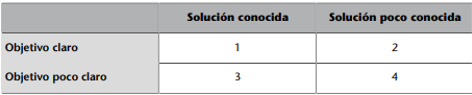
\includegraphics[width=1\textwidth]{img/4.TecnicasHerramientas/Clasificacion.png}
    \caption{Clasificación proyectos software \cite{pradel2013ingenieria}}
    \label{fig:clasificacionProyectos}
\end{figure}

El proyecto de desarrollo de una web para el seguimiento de la evolución de la marcha en pacientes con Párkinson se encuadraría dentro del Grupo 1. Dado que los obtjetivos y enfoque están claramente definidos, sería adecuado escoger el método de ciclo de vida cla´sico o en cascada \cite{pradel2013ingenieria}. Esta elección está justicada por la importancia de la sencillez de aplicación sobre la tolerancia al cambio. En otros casos, en los que la flexibilidad cobra más importancia, podría ser más conveniente aplicar métodos iterativos o ágiles.

\subsubsection{Ciclo de vida clásico o en cascada}
Este método de desarrollo software destaca por la sencillez de su aplicación y su forma de organización similar a una cadena de producción \cite{pradel2013ingenieria}.

Las etapas que conforman el desarrollo de un proyecto siguiendo este método son las mostradas en la Figura \ref{} y descritas \cite{pradel2013ingenieria} a continuación:
\begin{enumerate}
    \item Requisitos. Definir qué debe ser el producto a través de la recopilación y documentación de sus funcionalidades.
    \item Análisis y diseño. Definir los puntos de vista externo e interno del producto. Describir los componentes y cómo interaccionan entre sí.
    \item Implementación. Escribir el código de acuerdo con las especificaciones de análisis y diseño. Generar manuales y producto ejecutable.
    \item Pruebas. Comprobar que el producto final cumple con los requisitos.
    \item Mantenimiento. El producto se distribuye a los usuarios y se corrigen los defectos que estos encuentren.
\end{enumerate}

\begin{figure}[h]
    \centering
    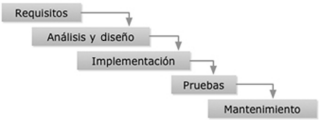
\includegraphics[width=0.7\textwidth]{img/4.TecnicasHerramientas/Cascada.png}
    \caption{Ciclo de vida en cascada \cite{pradel2013ingenieria}}
    \label{fig:cicloCascada}
\end{figure}


\subsection{Herramientas Software}



\subsection{Entornos de programación y programas}

\begin{itemize}
    \item \textbf{Visual Studio Code} (v1.84.2). Avanzado editor de código fuente disponible para Windows, macOS y Linux. Destaca por ser ligero y potente, ofreciendo soporte para JavaScript, TypeScript y Node.js, además de numerosas extensiones para otros lenguajes como Python y PHP \cite{VisualSt63:online}. Se puede obtener desde la página oficial \url{https://code.visualstudio.com/}.
    \item \textbf{XAMPP} (v8.2.0). Distribución de Apache que permite iniciar, detener y configurar de forma sencilla los servicios de MariaDB, PHP y Perl que contiene \cite{XAMPPIns2:online}. Descargar el instaldor desde \url{https://www.apachefriends.org/es/download.html} y ejecutar desde el ordenador.
    \item \textbf{Node.js} (v20.10.0). Entorno de ejecución de JavaScript del lado del servidor, es multiplataforma y de código abierto \cite{Nodejs—I6:online}. Instalación desde \url{https://nodejs.org/en} y comprobación a través de al ejecución del comando 'node -v' en el terminal cdm.
    \item \textbf{Node Package Manager} (v10.2.3). Es, por defecto, el sistema de gestión de paquetes de Node.js \cite{Nodejs—I6:online}. Obtención desde las opciones de instalación de Node.js. Se puede comprobar si la instalación ha sido correcta a través de la ejecución del comando 'npm -v' en el terminal cdm.
    \item \textbf{IDE Arduino} (v1.8.19). Entorno de programación de código abierto, sencillo y extensible a través de bibliotecas C++, para programar placas Arduino \cite{Arduino83:online}. Disponible en \url{https://www.arduino.cc/en/software}.
    \item \textbf{ChatGPT}. Herramienta de inteligencia artificial utilizada de apoyo en el desarrollo de código implementado para el funcionamiento del proyecto. Accesible desde \url{https://chat.openai.com/}
    \item \textbf{Balsamiq Wireframes} (v4.6.5). Herramienta para la creación de prototipos y maquetas de interfaces de forma rápida y clara \cite{Balsamiq0:online}. Hay una versión para escritorio disponible en \url{https://balsamiq.com/wireframes/desktop/}.
    \item \textbf{Diagramas.net} (v13.0.1). Herramienta en linea para la creación de diagramas y gráficos. Cuenta con diferentes opciones para su uso junto a VS Code, GitHub, Dropbox y herramientas similares de trabajo en equipo \cite{drawio51:online}. Accesible desde \url{https://www.drawio.com/}.
    \item \textbf{Lucidchart} (v1.163.3). Software de diagramación online que permite el trabajo individual y en equipo \cite{Lucid79:online}. Existe una versión gratis y otra más completa de pago. Se puede acceder desde \url{https://www.lucidchart.com/pages/es}.
    \item \textbf{GitHub} (v3.11.2). Repositorio en línea de código fuente que facilita el control de versiones y la colaboración en proyectos software mediante el sistema Git \cite{Git44:online}. Acceso desde Internet en el siguiente enlace: \url{https://github.com/}.
    \item \textbf{GitHub Desktop} (v3.3.6). Aplicación de escritorio que facilita el uso de Git y el trabajo con código almacenado en GitHub, mediante una interfaz gráfica de usuario \cite{Comenzar98:online}. Para instalar visita la página \url{https://desktop.github.com/}.

\end{itemize}


\subsubsection{Lenguajes de programación}
Una variedad de lenguajes han sido utilizados para la obtención de la página web:
\begin{itemize}
    \item Con soporte incorporado en VS Code: \textbf{HTML}, \textbf{JavaScript} y \textbf{CSS}.
    \item Con requisitos previos a su empleo en VS Code:
    \begin{itemize}
        \item \textbf{PHP}. Requiere una extensión de servidor PHP. Se ha empleado PHP Intelephense, disponible en las extensiones de VS Code.
        \item \textbf{Python} (v3.12.1). Para que su uso sea posible en VS Code debe ser instalado en el ordenador de trabajo desde \url{https://www.python.org/downloads/}, y añadir la extensión Python de Microsoft.
    \end{itemize}
    \item Sin requisitos adicionales: \textbf{SQL} y \textbf{Bootstrap}.
\end{itemize}

Además, ha sido necesario el uso del lenguaje \textbf{Arduino}. Basado en Wiring y similar a C++ \cite{Arduino83:online}. Se emplea dentro del Arduino IDE para crear el programa que se va a cargar en el microcontrolador Arduino UNO R3.

\subsubsection{Librerías y paquetes}
Librerías de Arduino:
\begin{itemize}
    \item \textbf{MPU6050}. Librería que permite realizar la lectura del MPU-6050 \cite{MPU605015:online}. Desarrollada por Jeff Rowberg y disponible en su repositorio de GitHub.
    \item \textbf{I2Cdev}. Mejora la estabilidad y eficiencia de la comunicación I2C \cite{MPU605015:online}. Se puede descargar como archivo zip desde el repositorio GitHub de Jeff Rowberg para su posterior subida a Arduino IDE.
    \item \textbf{Wire}. Necesaria para el funcionamiento de la librería I2Cdev. Permite la comunicación con dispositivos I2C \cite{WireArdu98:online}. Disponible en Arduino IDE en "Programa/Incluir librería".
    \item \textbf{SoftwareSerial}. Permite la comunicación, en este caso el envío de datos por Bluetooth, a través de pines digitales de la placa Arduino \cite{Software57:online}. Se puede incluir desde Arduino IDE en "Programa/Incluir librería".
    \item \textbf{LiquidCrystal\_I2C}. Requerida para el manejo de la pantalla LCD a través del módulo I2C \cite{LiquidCr9:online}. Posibilidad de instalar directamente en Arduino IDE siguiendo la ruta "Programa/Incluir librería/Administrar bibliotecas".
\end{itemize}

Paquetes Python:

Para la instalación ejecutar 'pip install pyserial requests' en la terminal de VS Code o cdm.
\begin{itemize}
    \item \textbf{PySerial}. Provee de comunicación serial a la aplicación Python , permitiendo la lectura y la escritura de datos \cite{pyserial96:online}.
    \item \textbf{Requests}. Librería HTTP para el envío de solicitudes de forma sencilla \cite{psfreque89:online}.
\end{itemize}

Paquetes Node.js:

Se deben instalar desde el terminal cdm situado en el directorio de mi proyecto node (en este caso en la carpeta 'Arduino Server').
\begin{itemize}
    \item \textbf{Express}. Framework que proporciona los mecanismos necesarios para el desarrollo de aplicaciones web \cite{Express10:online}. Se obtiene a través de la ejecución del comando 'npm install express'.
    \item \textbf{Body-Parser}. Librería que se utiliza con express para trabajar con datos de solicitudes como JSON y datos de formulario. El comando de instalación es 'npm install body\_parser'.
    \item \textbf{MySQL}. Utilizado para el manejo de la lógica que permite conectar la base de datos y el servidor de Node.js. Para proceder a la instalación ejecutar 'npm install mysql'.
    \item \textbf{CORS}. Se emplea con Express y sirve para habilitar el Intercambio de Recursos de Origen Cruzado (CORS) \cite{Intercam91:online} es decir, cuando el archivo html no se encuentra en el directorio de trabajo de Node.js. Instalación a través del comando 'npm install cors'.
\end{itemize}

\subsection{Tecnologías de comunicación}
La selección del método de conexión adecuado es vital para garantizar el óptimo funcionamiento del sistema y satisfacer las necesidades que este pretende abarcar. Para escoger la tecnología adecuada, es importante analizar las características de los principales métodos de comunicación disponibles para Arduino y aplicables a este proyecto: Ethernet, WiFi y Bluetooth.

\subsubsection{Ethernet}
Ethernet es una tecnología de comunicación que utiliza el protocolo Ethernet para permitir la conexión alámbrica de dispositivos electrónicos en una LAN (Local Area Network). También puede ser utilizada en una WAN (Wide Area Network) \cite{¿QuéesEt14:online} \cite{QuéesEth13:online}.

Permite el envío de datos y la conezión a internet de los equipos conectados por cable Ehternet a la red LAN de forma barata, diable, segura y a una muy alta velocidad \cite{¿QuéesEt14:online} \cite{QuéesEth13:online}.
\begin{itemize}
    \item \textbf{Shield Ethernet W5100} (Figura \ref{fig:moduloEthernet}). \\
    Es un módulo para Arduino en el que se diferencian dos partes:
    \begin{itemize}
        \item Chip W5100. Controlador de Ethernet que, sin necesidad de un Sistema Operativo, permite implementar la comunicación por internet en Arduino a través de la pila de protocolos TCP/IP \cite{Conectar3:online} para el envío de datos. Además, presenta un buffer interno de 16 Kbytes gracias al cual no consumirá memoria del microprocesador Arduino y que, junto con la pila de protocolos, conseguirá liberar a este de tareas \cite{Conectar3:online}.
        \item Lector microSD. Incorpora un lector microSD que puede servir para almacenar ficheros necesarios que le permitan actuar como servidor \cite{Conectar3:online}.
    \end{itemize}
    Ambos elementos comparten el bus SPI, requiriendo especial atención para evitar conflictos durante su uso conjunto \cite{Ethernet91:online}.
    \item Valoración. \\
    La tecnología Ethernet es alámbrica, lo que supone una gran desventaja si se aplica a este proyecto. No permite cumplir los objetivos principales de aumento de la autonomía y comodidad del usuario.
\end{itemize}

\begin{figure}[h]
    \centering
    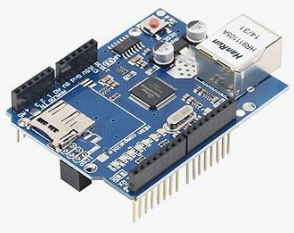
\includegraphics[width=0.5\textwidth]{img/4.TecnicasHerramientas/Ethernet.png}
    \caption{Shield Ethernet W5100 \cite{Ethernet92:online}}
    \label{fig:moduloEthernet}
\end{figure}

\subsubsection{WiFi}
WiFi es una tecnología de red de área local inalámbrica (WLAN) que, a través de radiofrecuencia \cite{WhatisWi11:online}, proporciona acceso a Internet a todos los dispositivos conectados y al mismo tiempo les permite interaccionar entre sí \cite{¿Quéesla82:online}. Todo el proceso de comunicación está definido por los protocolos del estándar IEE 802.11 \cite{¿Quéesla82:online}\cite{WhatisWi11:online}.

La conexión a Internet se consigue a través de un router inalámbrico que emite una señal dentro de cuyo alcance cualquier dispositivo, también inalámbrico, podrá conectarse \cite{¿Quéesla82:online}. 
\begin{itemize}
    \item \textbf{Módulo WiFi ESP8266 ESP01 }(Figura \ref{fig:moduloWiFi}). \\
    El módulo para Arduino está conformado por la memoria Flash, principal diferencia entre los diferentes módulos ESP8266; y el SoC (System on Chip) ESP8266, que agrupa diversos componentes entre los que destacan un procesador de 32 bits y un chip WiFi que implementa protocolos TCP/IP \cite{ESP8266l93:online}. Además, destaca entre el resto de la familia ESP8266 debido a su reducido tamaño y bajo precio.

    \item Valoración. \\
    Su principal ventaja frente a la conexión Ethernet es que al ser inalámbrica permite mayor comodidad y movilidad, pero esto también se traduce en una reducción de la seguridad y la velocidad, que además presentará mayores fluctuaciones y por tanto una menor fiabilidad \cite{WiFivsEt71:online}. De todos modos, para este proyecto, la conexión inalámbrica se considera una prioridad, por lo que el empleo de tecnología WiFi sería más adecuado que el de Ethernet.
\end{itemize}

\begin{figure}[h]
    \centering
    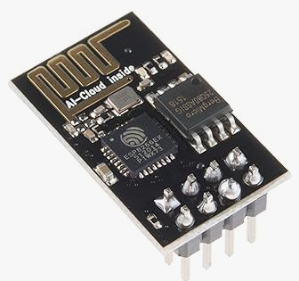
\includegraphics[width=0.3\textwidth]{img/4.TecnicasHerramientas/WiFi.png}
    \caption{Shield Ethernet W5100 \cite{WiFi1:online}}
    \label{fig:moduloWiFi}
\end{figure}

\subsubsection{Bluetooth}
Bluetooth es una tecnología inalámbrica de corto alcance que utiliza ondas de radio para la transmisión de datos (principalmente paquetes pequeños) y la conexión directa entre dos dispositivos (hosts) sin la necesidad de una infraestructura de red \cite{¿Quéesla6:online}.

El emparejamiento de dos dispositivos mediante bluetooth es un proceso simple que puede llevarse a cabo de forma manual y en ocasiones automática. La conexión se caracteriza por el salto de los dispositivos emparejados entre los diferentes canales en búsqueda de la menor interferencia \cite{¿Cómofun38:online}, lo que se denomina salto en frecuencia y permite un desempeño consistente y de baja latencia.

\begin{itemize}
    \item \textbf{Módulo Bluetooth HC-05} (Figura \ref{fig:moduloBluetooth}). \\
    Permite la conexión de Arduino con otro dispositivo de forma muy sencilla ya que es similar a utilizar un puerto serie normal. Su principal característica es que actúa como master y server \cite{Conectar13:online}, lo que significa que permite tanto iniciar como recibir comunicaciones. Por este motivo se elige frente al módulo HC-06, que únicamente permite recibir \cite{Conectar13:online}.

    \item Valoración. \\
    Si se compara la conexión bluetooth con la red WiFi una de las mayores diferencias es el alcance máximo, siendo mayor el de la tecnología WiFi. Además, ambas tecnologías son inalámbricas y conectan dispositivos entre sí, pero, mientras que el Bluetooth se emplea preferiblemente para la conexión de periféricos y dispositivos debido a su mayor potencia, la WiFi se utiliza para dar acceso a Internet ya que se caracteriza por una mayor velocidad \cite{Diferenc89:online}.
\end{itemize}

\begin{figure}[h]
    \centering
    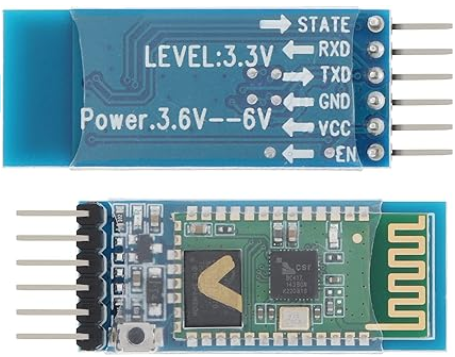
\includegraphics[width=0.3\textwidth]{img/4.TecnicasHerramientas/HC-05.png}
    \caption{Shield Ethernet W5100 \cite{HC0536:online}}
    \label{fig:moduloBluetooth}
\end{figure}

\subsubsection{Selección tecnología}
Con el fin de escoger la tecnología más adecuada para cumplir con los requisitos del proyecto, se realizó un análisis en profundidad de cada una de ellas. La elección del Bluetooth se basa en dos razones principales:
\begin{enumerate}
    \item Ventajas de la conexión inalámbrica para la comodidad de uso. Ethernet es la única tecnología que no cumple con este requirimiento.
    \item Priorizar la conexión entre dispositivos. La WiFi, además de permitir conexión inalámbrica entre dispositivos, proporciona a nuestro dispositivo una conexión a Internet innecesaria y que supone complicaciones adicionales. Esto proporciona una ventaja al Bluetooth, que destaca por su simplicidad y eficiencia en la conexión.
\end{enumerate}

\subsection{Herramientas Hardware}
Partiendo del prototipo desarrollado en \cite{saragonz91:online}, se ha desarrollado una versión básica que implementa el envío de datos de forma inalámbrica a través de un módulo Bluetooth. Se proporciona autonomía completa al dispositivo para su uso en el desarrollo de pruebas.

En este apartado se incluye una breve descripción de todos los componentes hardware utilizados.
\begin{itemize}
    \item \textbf{Microcontrolador Arduino UNO R3} (Figura \ref{fig:arduinoUNO}.\\
    Placa microcontroladora basada en el ATMega328P y que dispone de entradas y salidas para pines tanto digitales como analógicos \cite{ArduinoUNO82:online}. Es sencilla de programar utilizando Arduino IDE y facilita la carga de programas mediante conexión USB.

    \begin{figure}[h]
        \centering
        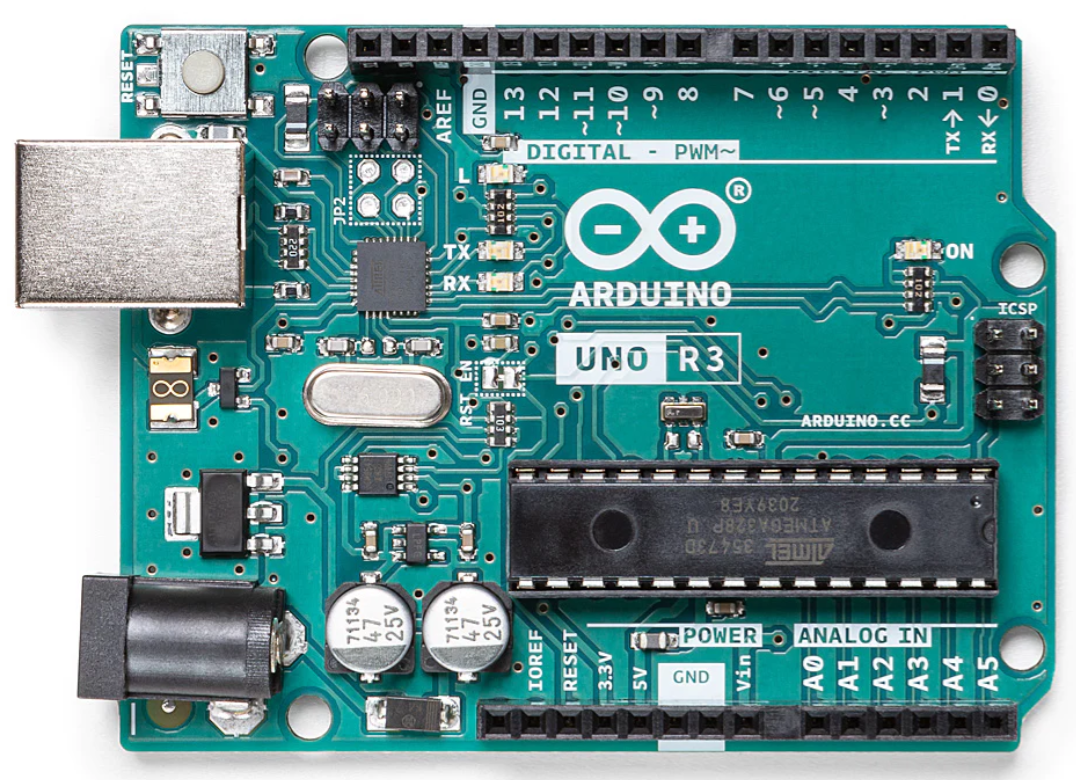
\includegraphics[width=0.5\textwidth]{img/4.TecnicasHerramientas/ArduinoUNO.png}
        \caption{Microcontrolador Arduino UNO R3. \cite{ArduinoUNO82:online}}
        \label{fig:arduinoUNO}
    \end{figure}
    
    \item Acelerómetro + Giroscopio MPU-6050 (Figura \ref{fig:mpu}).
    Unidad de Medición Inercial (IMU) de muy bajo precio, cuya comunicación se puede realizar mediante bus I2C o por SPI de forma sencilla, y que incluye 6 ejes (3 del giroscopio y 3 del acelerómetro \cite{MPU605015:online}. Una de sus principales ventajas es su reducido coste.
    
    \begin{figure}[h]
        \centering
        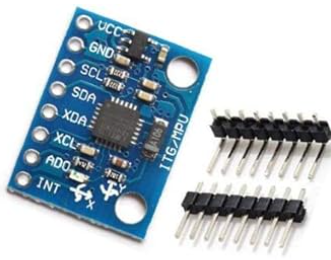
\includegraphics[width=0.3\textwidth]{img/4.TecnicasHerramientas/MPU6050.png}
        \caption{Sensor MPU-6050. \cite{MPU6050Amazon396:online}}
        \label{fig:mpu}
    \end{figure}
    
    \item Display LCD 16x2 con interfaz I2C (Figura \ref{fig:lcd}). \\
    En la pantalla lcd se mostrarán datos enviados por el programa de Arduino para que el usuario pueda consultarlos mientras la actividad está en curso, a pesar de que también se mostrarán en la web. La interfaz I2C simplifica el número de conexiones del módulo lcd con Arduino y añade funcionalidades entre las que se encuentran el control del brillo y ajuste del contraste \cite{16x2LCDd27:online}.
    
    \begin{figure}[h]
        \centering
        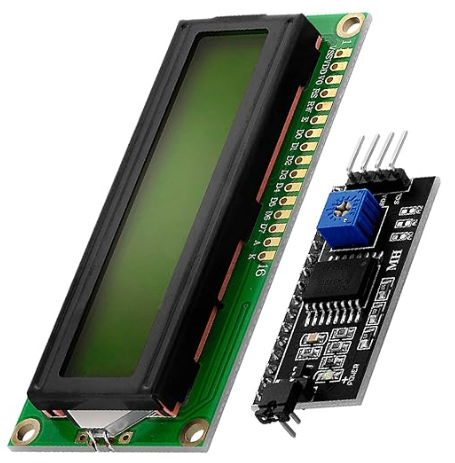
\includegraphics[width=0.3\textwidth]{img/4.TecnicasHerramientas/LCDI2C.png}
        \caption{Display LCD 16x2 con interfaz I2C. \cite{lcdFoto88:online}}
        \label{fig:lcd}
    \end{figure}

    \item \textbf{Módulo Bluetooth HC-05} (Figura \ref{fig:moduloBluetooth}). \\
    Proporciona una forma sencilla de conexión para el envío de datos entre Arduino y otro dispositivo, contando con la ventaja tener funcionalidad master y server \cite{Conectar13:online}.
    
    \item \textbf{Pulsadores} (Figura \ref{fig:pulsador}). \\
    Incluidos en el programa Arduino de tal forma que permitan el inicio y finalización de la actividad de recogida de datos.
    
    \begin{figure}[h]
        \centering
        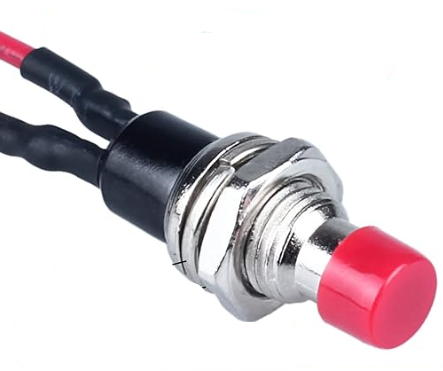
\includegraphics[width=0.2\textwidth]{img/4.TecnicasHerramientas/Pulsador.png}
        \caption{Pulsador. \cite{Pulsador32:online}}
        \label{fig:pulsador}
    \end{figure}
    
    \item \textbf{Resistencias} necesarias para el correcto montaje de los pulsadores.
    
    \item \textbf{Cables} para realizar las conexiones pertinentes.
\end{itemize}

\subsubsection{Mejoras hardware}
En este trabajo se pretendía, además de lograr la comunicación, realizar unas pequeñas mejoras que permitieran el funcionamiento del prototipo de forma autónoma y con la mayor comodidad posible para el paciente. Se realizó un trabajo de soldadura para asegurar las conexiones entre todos los componentes. Los elementos hardware empleados son los que se describen a continuación.
\begin{itemize}
    \item \textbf{Caja para prototipos} (Figura \ref{fig:cajaPrototipos}). \\
    Almacena todo el hardware necesario para el funcionamiento del prototipo, excepto el módulo MPU-6050, que se ubica en el tobillo izquierdo. Fabricada con un plástico resistente que protejerá el microprocesador y las conexiones entre todos los componentes. Tiene perforaciones diseñadas exclusivamente para los siguientes propósitos:
    \begin{itemize}
        \item Visualización del display LCD.
        \item Acceso a pulsadores e interruptor.
        \item Permitir la conexión USB del microprocesador Arduino UNO para la carga de programas.
        \item Sujección de una parte del conector 5 pines.
    \end{itemize}

    \begin{figure}[h]
        \centering
        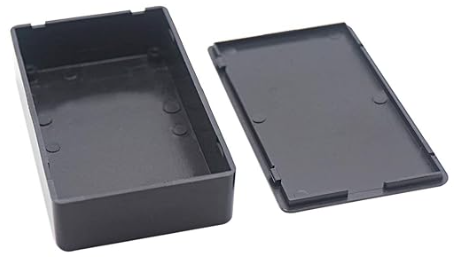
\includegraphics[width=0.5\textwidth]{img/4.TecnicasHerramientas/CajaPrototipos.png}
        \caption{Caja para prototipos \cite{CajaProt627:online}}
        \label{fig:cajaPrototipos}
    \end{figure}
    
    \item \textbf{Batería recargable de 9V y conector de batería} (Figura \ref{fig:bateria}).\\
    Provee una fuente de alimentación externa que, junto al módulo Bluetooth, permite la autonomía total del prototipo.

    \begin{figure}[h]
        \centering
        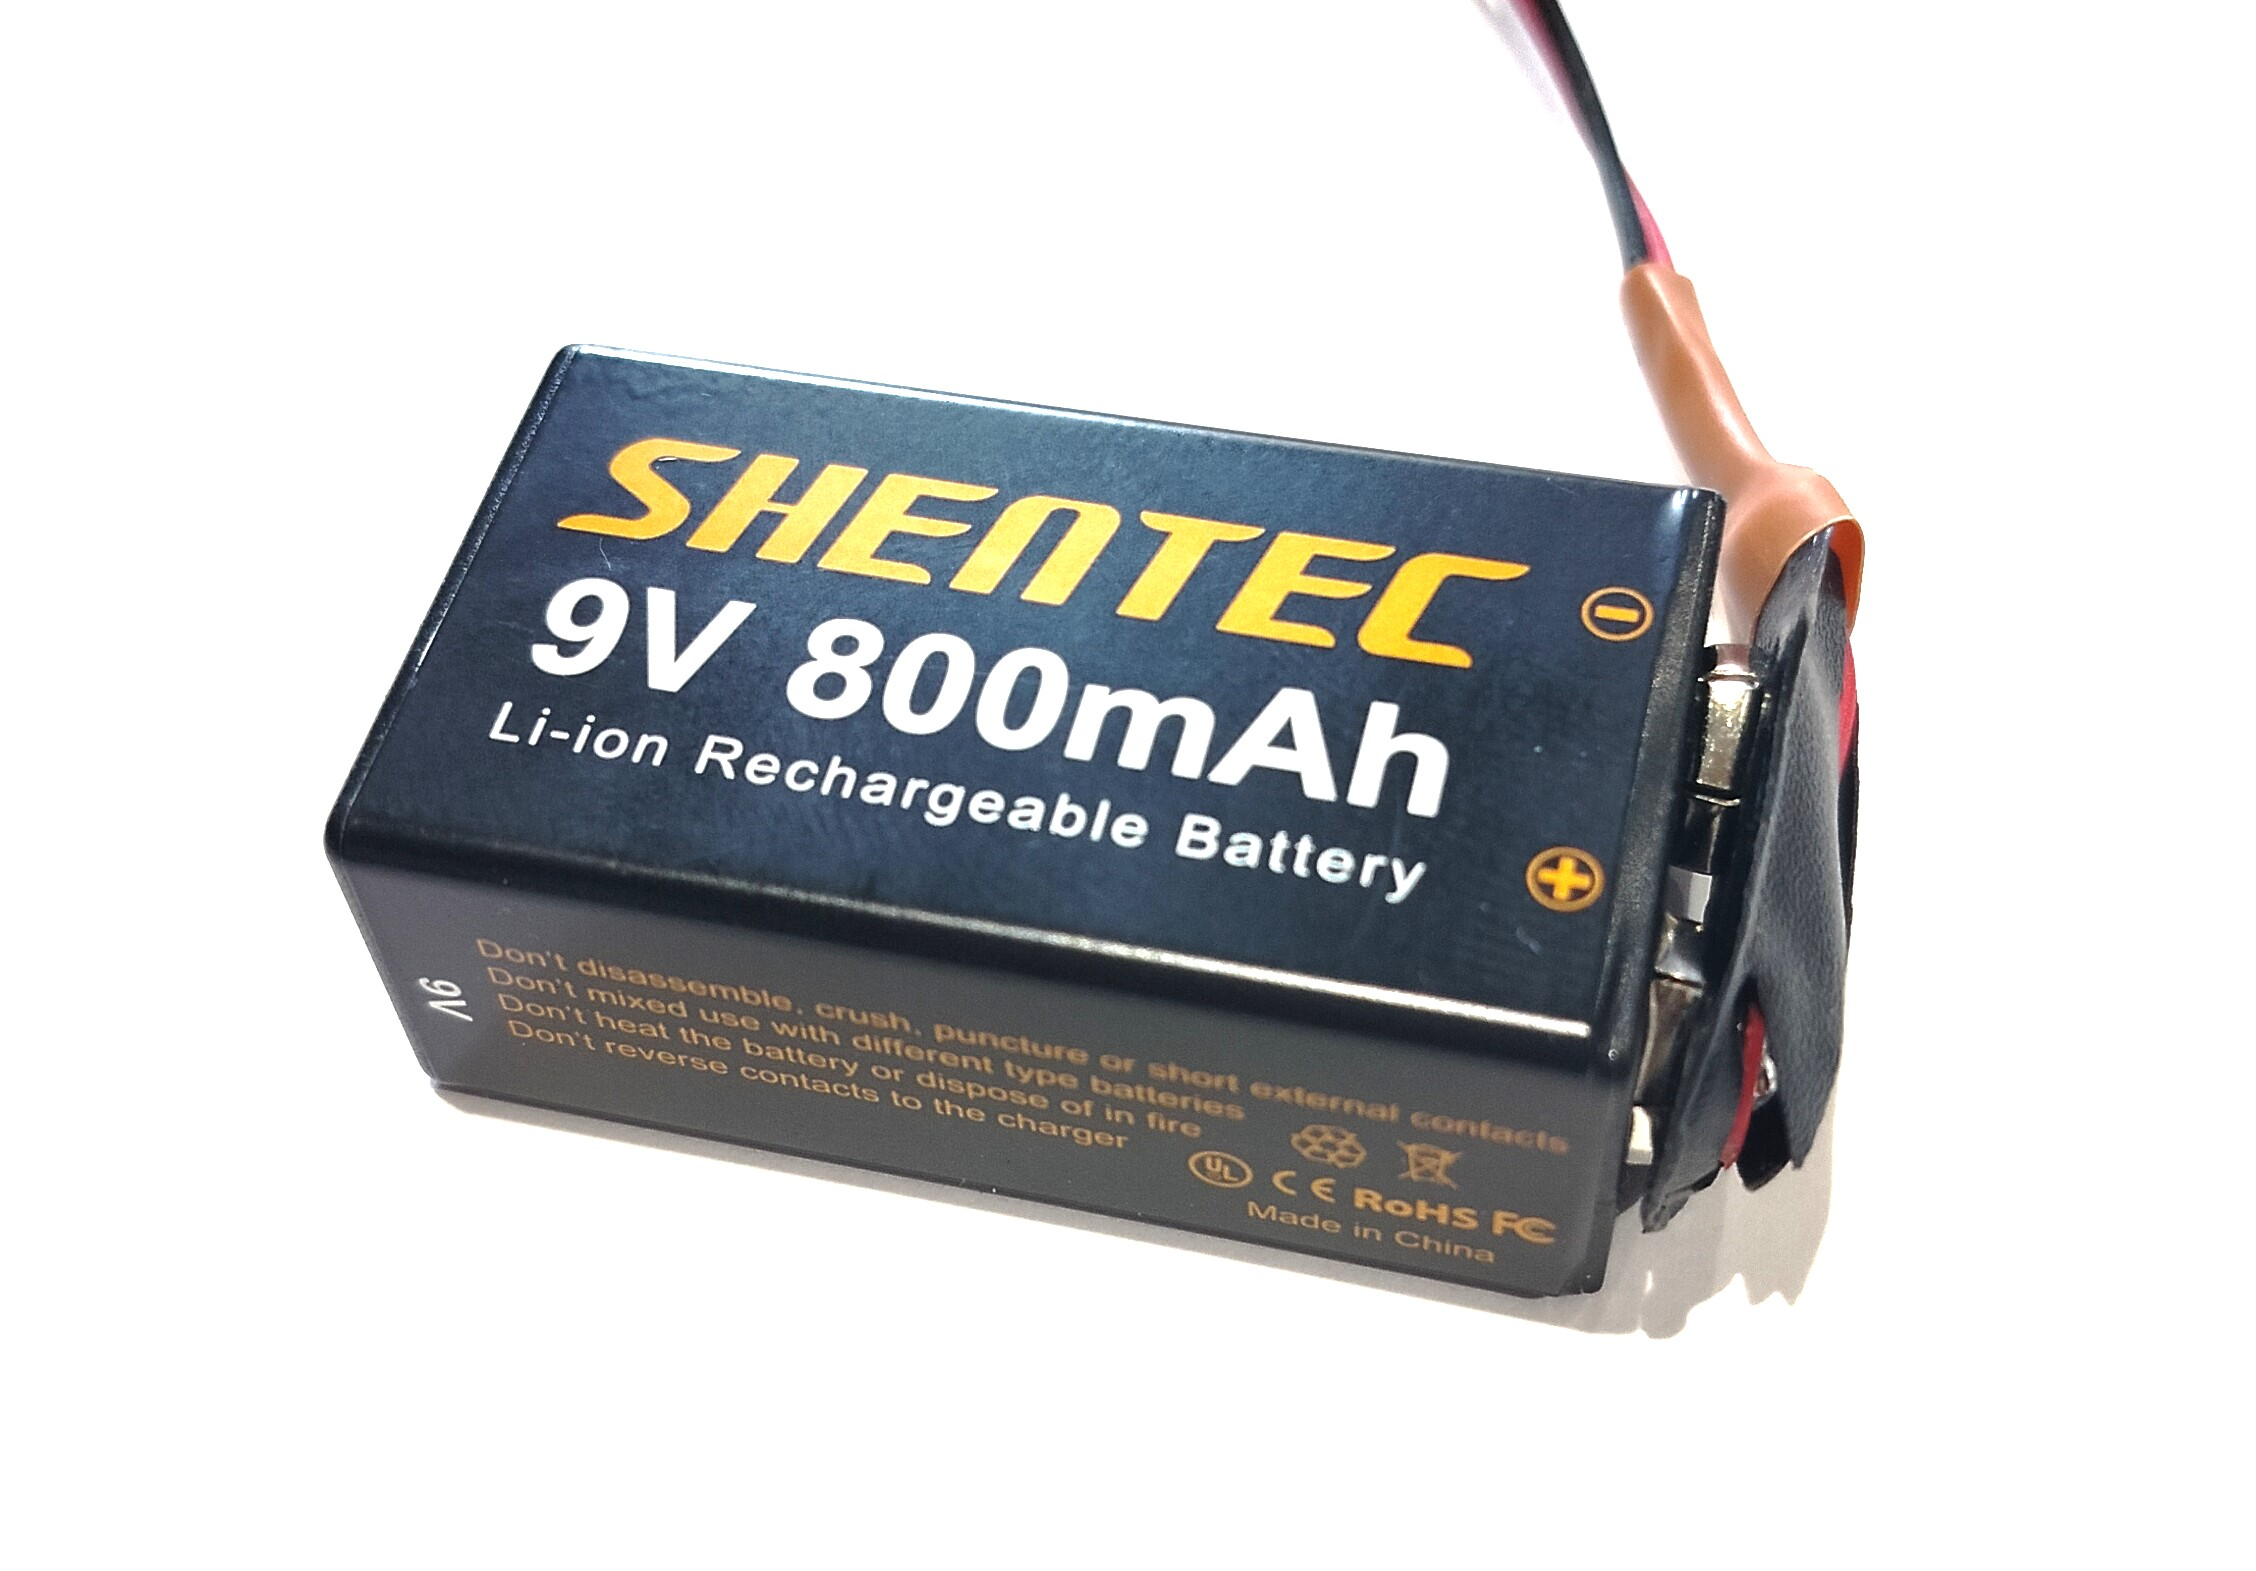
\includegraphics[width=0.5\textwidth]{img/4.TecnicasHerramientas/Bateria.jpg}
        \caption{Batería 9V con conector. Fuente propria}
        \label{fig:bateria}
    \end{figure}
    
    \item \textbf{Interruptor} (Figura \ref{fig:interruptor}).\\
    Mecanismo de encendido y apagado, controla el flujo de energía que llega al sistema desde la batería externa.

    \begin{figure}[h]
        \centering
        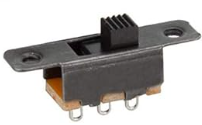
\includegraphics[width=0.3\textwidth]{img/4.TecnicasHerramientas/Interruptor.png}
        \caption{Interruptor deslizante. \cite{Interruptor42:online}}
        \label{fig:interruptor}
    \end{figure}

    \item \textbf{Conector 5 pines} (Figura \ref{fig:conector5pines}).\\
    Este conector macho y hembra permite la conexión y desconexión del módulo MPU-6050 del sistema. Proporciona dos partes separables: el sensor y la caja de prototipos con el resto del hardware. Es una funcionalidad que facilita el almacenamiento y uso del prototipo. 

    \begin{figure}[h]
        \centering
        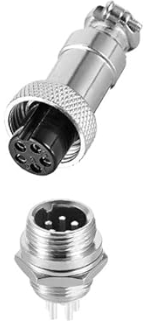
\includegraphics[width=0.2\textwidth]{img/4.TecnicasHerramientas/Conector5pines.png}
        \caption{Conector 5 pines. \cite{Conector5P61:online}}
        \label{fig:conector5pines}
    \end{figure}
    
    \item \textbf{Cable multihilo flexible} (Figura \ref{fig:cableMultihilo}).\\
    El cable contiene un mínimo de cuatro hilos y debe ser flexible para asegurar una completa libertad de movimiento al usuario. Conecta el módulo MPU-6050 a un extremo del conector 5 pines.

    \begin{figure}[h]
        \centering
        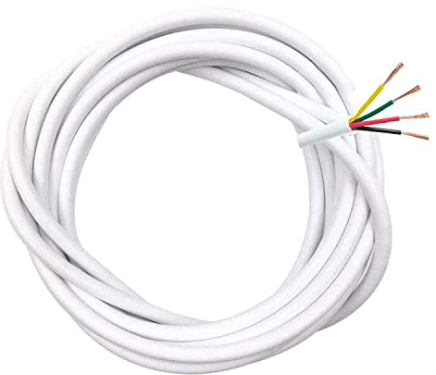
\includegraphics[width=0.4\textwidth]{img/4.TecnicasHerramientas/CableMultihilo.png}
        \caption{Cable multihilo flexible. \cite{Cable41:online}}
        \label{fig:cableMultihilo}
    \end{figure}
    
    \item \textbf{Proto Shield} (Figura \ref{fig:shield}).\\
    Fácilmente acoplable al microprocesador, permite la construcción de circuitos mediante soldadura para una mayor seguridad en la conexión de los elementos que componen el prototipo.

    \begin{figure}[h]
        \centering
        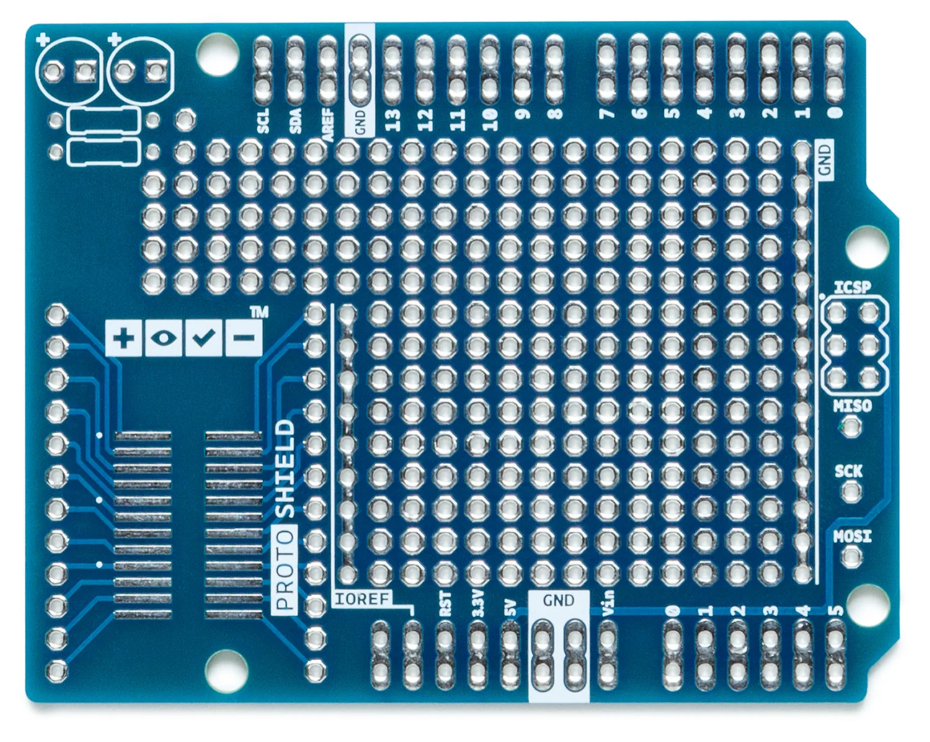
\includegraphics[width=0.4\textwidth]{img/4.TecnicasHerramientas/Protoshield.png}
        \caption{Proto Shield. \cite{ProtoShi18:online}}
        \label{fig:shield}
    \end{figure}
    
    
\end{itemize}




\capitulo{5}{Resultados}

\section{Resumen de resultados.}

Breve resumen de los resultados. En caso de ser un trabajo muy experimental, los resultados completos pueden aparecer en su anexo correspondiente.

Debería haber una correspondencia entre los objetivos y los resultados explicados en esta sección

\section{Discusión.}

Discusión y análisis de los resultados obtenidos.
\capitulo{6}{Conclusiones}

Todo proyecto debe incluir las conclusiones que se derivan de su desarrollo. Éstas pueden ser de diferente índole, dependiendo de la tipología del proyecto, pero normalmente van a estar presentes un conjunto de conclusiones relacionadas con los resultados del proyecto y un conjunto de conclusiones técnicas. 



\section{Aspectos relevantes.}



-> La exactitud se vae afectada por la poca fiabilidad del registro y rpocesamiento de los datos en el arduino.




Este apartado pretende recoger los aspectos más interesantes del \textbf{desarrollo del proyecto}, comentados por los autores del mismo.

Debe incluir los detalles más relevantes en cada fase del desarrollo, justificando los caminos tomados, especialmente aquellos que no sean triviales. 

Puede ser el lugar más adecuado para documentar los aspectos más interesantes del proyecto y también los resultados negativos obtenidos por soluciones previas a la solución entregada.

Este apartado, debe convertirse en el resumen de la experiencia práctica del proyecto, y por sí mismo justifica que la memoria se convierta en un documento útil, fuente de referencia para los autores, los tutores y futuros alumnos.





\capitulo{7}{Lineas de trabajo futuras}

Este proyecto se concibe como la ampliación de un trabajo previo \cite{saragonz91:online}, avanzando hacia la creación de un prototipo autónomo capaz de trabajar en coordinación con una aplicación software. Se ha logrado el objetivo general mediante el desarrollo de una página web, pero existen aspectos que requieren la continuación del trabajo de mejora. Entre estas mejoras destacan el fortalecimiento de la seguridad, el desarrollo de un diseño web más atractivo y el lanzamiento de la página web para su acceso desde cualquier dispositivo, ya que actualmente únicamente opera en modo local. Además, se debe considerar la posibilidad de mejorar la comunicación en tiempo real mediante la implementación de WebSockets, así como el desarrollo de una aplicación móvil que complemente a la plataforma web.

En cuanto a las funcionalidades del sistema, se propone mejorar el procesamiento de datos y obtener nuevas mediciones con el fin de generar unas estadísticas clínicas más precisas y relevantes. Esto incluye la implementación de un registro de la administración de medicamentos, ofrecer la posibilidad de registrar actividades sin que el Bluetooth esté conectado, y facilitar el proceso de calibración del sensor encargado de la monitorización.

A pesar de que no era un objetivo principal, este proyecto ha logrado una mejora en el prototipo hardware que facilita la realización de pruebas, pero no se han satisfecho necesidades hardware identificadas en la versión anterior. Además, se han detectado nuevos requerimientos. Las posibilidades de trabajo sobre el dispositivo, van desde la implementación de un sistema de alerta para episodios de congelación de la marcha, hasta mejoras en la precisión del sensor MPU6050 y añadir otro adicional para la pierna derecha.

En el Anexo \textit{Instrucciones para la modificación o mejora del proyecto}, se incluyen comentarios de interés y se detallan a fondo cada uno de los aspectos susceptibles de mejora mencionados en este apartado.


\bibliographystyle{apalike}
\bibliography{bibliografia}

\end{document}
